\subsection{Speed Regulation on NAO}

\label{sec:nao_walking}

%An approach to control the walking speed of NAO was achieved by
%using the Human-Inspired Control (HIC) and Context-Free Motion Grammar (CFG).

The NAO is a small bipedal robot produced by Aldebaran Robotics.  It
contains an on-board Intel Atom PC running a minimal Linux
distribution and includes the NAOqi framework to control the robot.
User code is loaded into the NAOqi process as dynamic library modules.
We used Ach to implement Human-Inspired Control \cite{Ames:NAO:2012}
on the NAO.  The Human-Inspired Control approach achieves provably
stable, human-like walking on robots by identifying key parameters in
human gaits, and transferring those to the robot through an
optimization process \cite{Ames11}.  To implement this approach,
real-time control software to produce the desired joint angles must
run on the NAO's internal computer.

% speed based on theoretically stable periodic orbits. The
% Human-Inspired Control provides a set of control parameters to
% generate the joint trajectories for stable walking with a certain
% fixed walking speed.

The NAOqi framework provides an interface to the robot's hardware;
however, it presents some specific challenges for application
development -- and for the implementation of Human-Inspired Control in
particular.  NAOqi is slow and memory-intensive, consuming at idle
15\% of available CPU time and 20\% of available memory.
Additionally, real-time user code must run as a callback function,
which is awkward for the desired controller implementation.  Using Ach
to move the controller to a separate process improves the
implementation.


A multi-process software design, \autoref{fig:naoprogram}, addresses
the shortcomings of NAOqi. In this approach, two separate processes,
{\tt motionControl} and {\tt logger/debugger}, interface with NAOqi
through the Ach IPC library. Two Ach channels are used: a control
channel for command data from {\tt motionControl} and a feedback
channel for sensor data from NAOqi. In order connect NAOqi with these
other processes via Ach, a minimal local module, {\tt libamber}, loads
into the NAOqi process, and all nonessential modules of NAOqi are
deactivated.  The {\tt libamber} module communicates over the two Ach
channels using the periodic, 10ms callback function provided by the
NAO's Device Communication Manager (DCM). When the DCM reads a new set
of sensor values, it notifies {\tt libamber} using a post-process
callback function. After that, {\tt libamber} writes the newly-read
sensor values into the feedback channel.  Before the DCM transmits
desired actuator values to the hardware, it calls a pre-process
callback function. On this event, {\tt libamber} reads the newest
command values from the control channel and then sends it to NAO's
servomotors through the DCM.

The {\tt motionControl} process produces the desired angles for
human-like walking on NAO. This process contains two core modules,
{\tt motionParser} and {\tt trajectoryGenerator}. The {\tt
  motionParser} \cite{dantam2013tro} contains a Finite State Machine
(FSM) which parses the robot's current state based on the newest
sensor data read from the feedback channel. Then {\tt
  trajectoryGenerator} computes the desired joint angles to yield
human-like walking on the NAO \cite{jars_2012_psa_01}.

The {\tt logger/debugger} process records data from both Ach
channels. This shows robot state during operation and allows offline
analysis of the data.  Since this process runs at lower priority than
both {\tt motionControl} and NAOqi, it does not affects the real-time
control of the robot.

In addition to steady-state fixed speed walking, we implement
speed-controlled walking on the NAO by tracking a stable sequence of
speed transitions. The {\tt Supervisor Generator} process computes a
\emph{supervisor} for a stable path of transitions to the desired
speed, adjusting the behavior of the {\tt motionParser}.  These two
processes communicate over two Ach channels: {\tt chan\_vel} contains
the current walking speed of the robot at the end of each step, and
{\tt chan\_super} contains the active supervisor for the target speed.


Adopting this multi-process design based on the Ach IPC library
enhances the robustness and efficiency of Human-Inspired Control on
the NAO.  Each process runs independently, so an error in a
non-critical process, such as {\tt logger/debugger}, cannot affect
other processes, eliminating a potential failure.  The user processes
can be stopped and started within only a few seconds.  In contrast,
NAOqi takes about 15 seconds to start. The independence of processes
means NAOqi need not be restarted so long as {\tt libamber} is
unchanged.  Since {\tt libamber} is a minimal module, only interfacing
with the Ach channels and accessing the NAO's hardware, it can be
reused unmodified for different applications on the NAO. Different
projects can run different controller processes, using Ach and {\tt
  libamber} to access NAO's hardware, all without restarting the NAOqi
process.  In addition, using standard debugging tools such as GDB is
much easier since the user code can be executed within the debugger
independently of the NAOqi framework.  Thus, converting the NAO's
control software to a multi-process design simplified development and
improved reliability.



\begin{figure}
  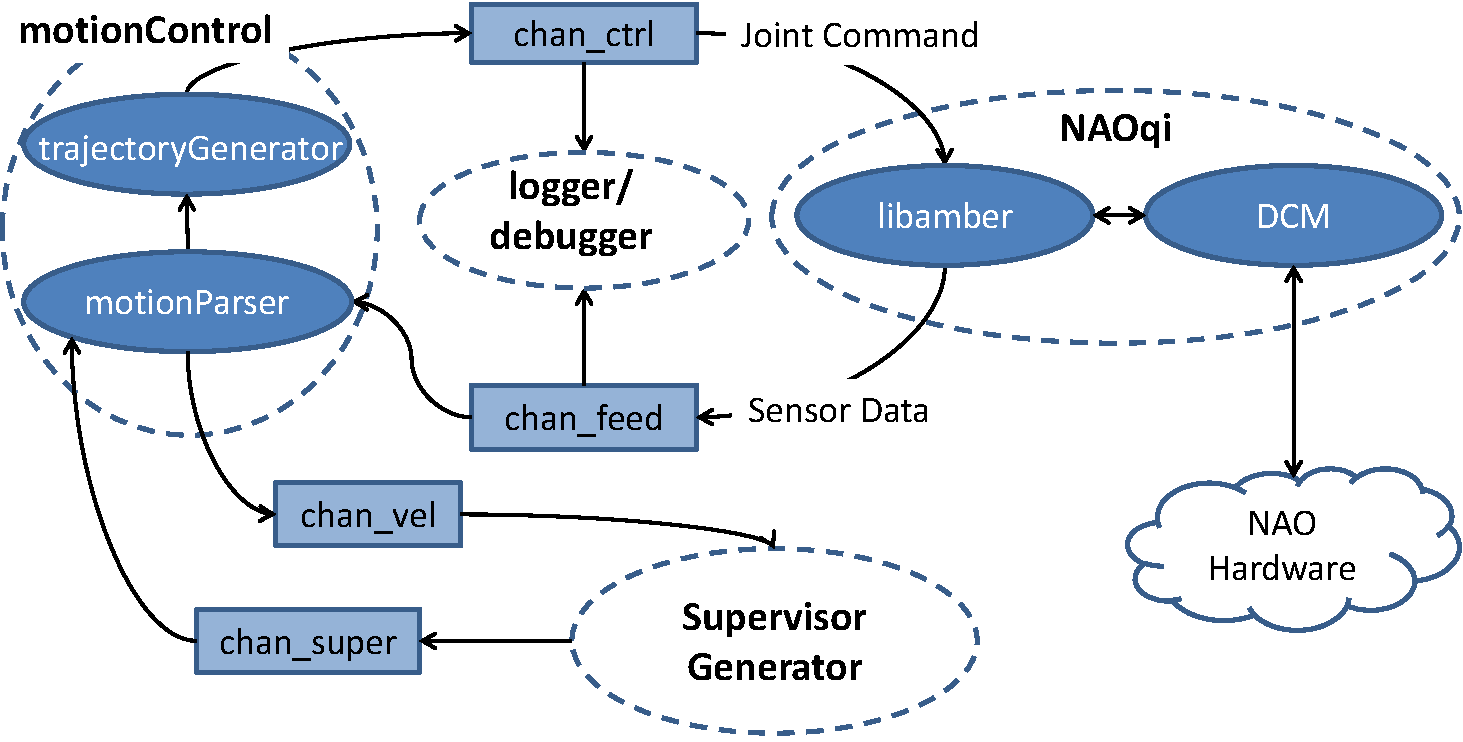
\includegraphics[width=.5\textwidth]{fig/naoprogram}
  \caption{Block diagram of primary software components on NAO.
  Ovals with dashed line are system processes, blue ovals with solid
line are modules contain within process, and rectangles are Ach channels.}
  \label{fig:naoprogram}
  \vspace{-2.0em}
\end{figure}

%%% Local Variables:
%%% mode: latex
%%% TeX-master: "ach.tex"
%%% End:
